\documentclass{article}
\usepackage{amsmath}
\usepackage{graphicx}
\usepackage{float}
\title{ENPH 353 Exercise - \LaTeX}
\author{Keegan Kelly}
\date{\today}



\begin{document}
    \maketitle
    \section{Getting Started}
    \textbf{Hello World!} 
    
    Here is a sample exercise in \LaTeX that will give you a chance to do some basic work.  Use the \verb+\usepackage{amsmath}+ and usepakage{graphicx} codes in the preamble so that we can include external figures and use more advanced equations.  By using the verb command, we can show how commands are typed.
    
    I would use this program when I want to write a lot of equations.  I can write in line math such as $a^2+b^2=c^2$. I can also give equations their own space using \verb+\begin{equation} x=... \end {equation}:+ 
    \begin{equation}
        x = \frac{-b \pm\sqrt{b^2-4ac}}{2a}
    \end{equation}
    
   The \verb+\begin{align} x&=y\\z&=y2 \end{align}+ command allows for sev-
eral equations to be lined up vertically. “Maxwell’s equations” are named for
James Clerk Maxwell and are as follows:
   \begin{align}
    \vec{\nabla} \cdot \vec{E} &= \frac{\rho}{\epsilon_0} \label{eq1}\\
    \vec{\nabla}\cdot\vec{B} &= 0 \label{eq2}\\
    \vec{\nabla}\times \vec{E} &= -\frac{\partial\vec{B}}{\partial t} \label{eq3}\\
    \vec{\nabla}\times \vec{B} &= \mu_0 \left(\epsilon_0\frac{\partial\vec{E}}{\partial t}+ \vec{J}\right) \label{eq4}
 \end{align}    

\noindent    
Equations \ref{eq1}, \ref{eq2}, \ref{eq3}, and \ref{eq4} are some of the most important in Physics. I labelled
each one using \verb+\label{name}+, and then referenced them using \verb+\ref{name}+.


\begin{figure}[H]
    \centering
    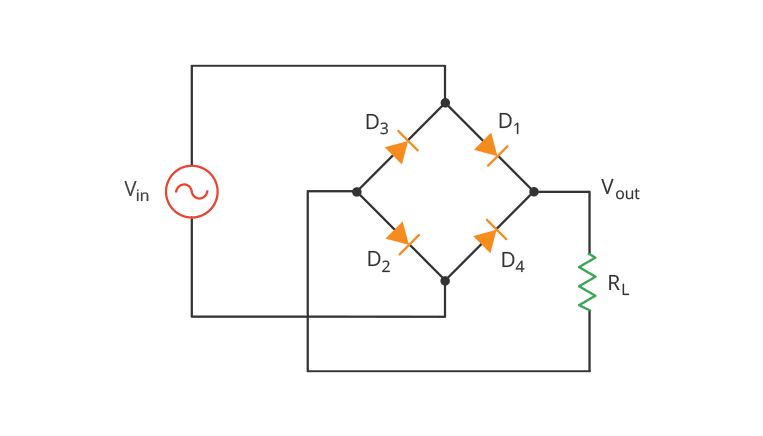
\includegraphics[width=0.5\textwidth]{Fullwave-Bridge-Rectifier.png}
\caption{Circuit diagram of a full bridge rectifier.}
\end{figure}

\end{document}